% LaTeX Article Template - customizing page format
%
% LaTeX document uses 10-point fonts by default.  To use
% 11-point or 12-point fonts, use \documentclass[11pt]{article}
% or \documentclass[12pt]{article}.
\documentclass{article}

% Set left margin - The default is 1 inch, so the following 
% command sets a 1.25-inch left margin.
\setlength{\oddsidemargin}{0.25in}

% Set width of the text - What is left will be the right margin.
% In this case, right margin is 8.5in - 1.25in - 6in = 1.25in.
\setlength{\textwidth}{6in}

% Set top margin - The default is 1 inch, so the following 
% command sets a 0.75-inch top margin.
\setlength{\topmargin}{-0.25in}

% Set height of the text - What is left will be the bottom margin.
% In this case, bottom margin is 11in - 0.75in - 9.5in = 0.75in
\setlength{\textheight}{8in}
\usepackage{fancyhdr}
\usepackage{float}
\usepackage{mathtools}
\usepackage{amsmath}
\usepackage{amssymb}
\usepackage{graphicx}
\usepackage{float}
\DeclarePairedDelimiter\Floor\lfloor\rfloor
\DeclarePairedDelimiter\Ceil\lceil\rceil
\graphicspath{ {./} }
\setlength{\parskip}{5pt} 
\pagestyle{fancyplain}
% Set the beginning of a LaTeX document
\begin{document}

\lhead{Drew Remmenga MATH 408}
\rhead{Project \#5}
%\lhead{Independent Study}
%\rhead{R Lab}

\begin{enumerate}

\item 
	\begin{enumerate}
	\item
	\item Figure
	\begin{figure}[H]
	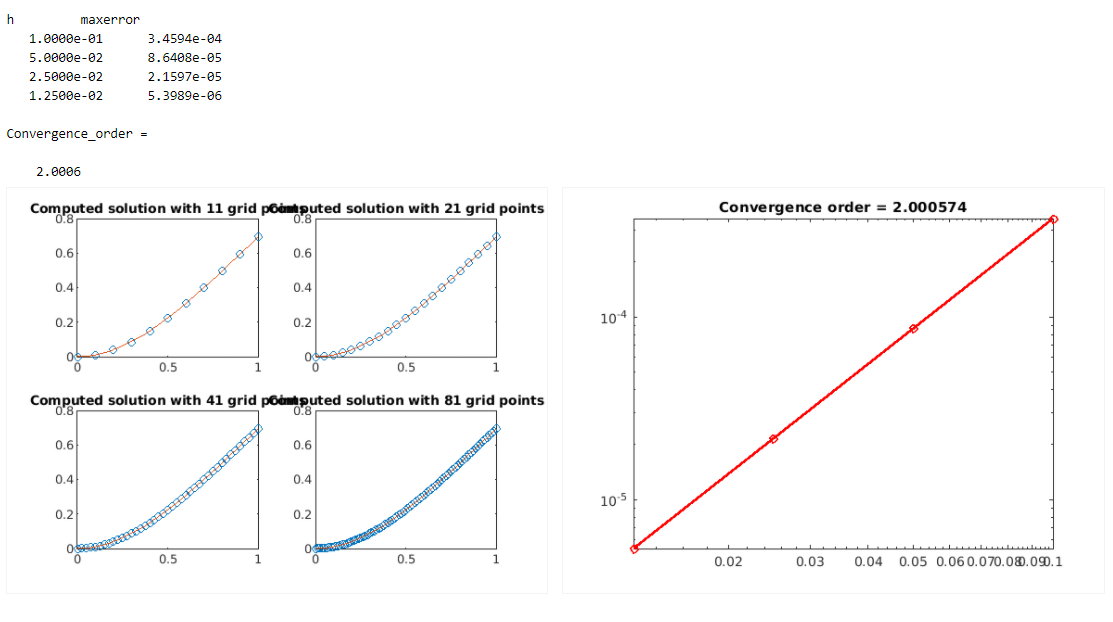
\includegraphics[scale=.5]{1b.PNG}
	\end{figure}
	\item Figure
	\begin{figure}[H]
	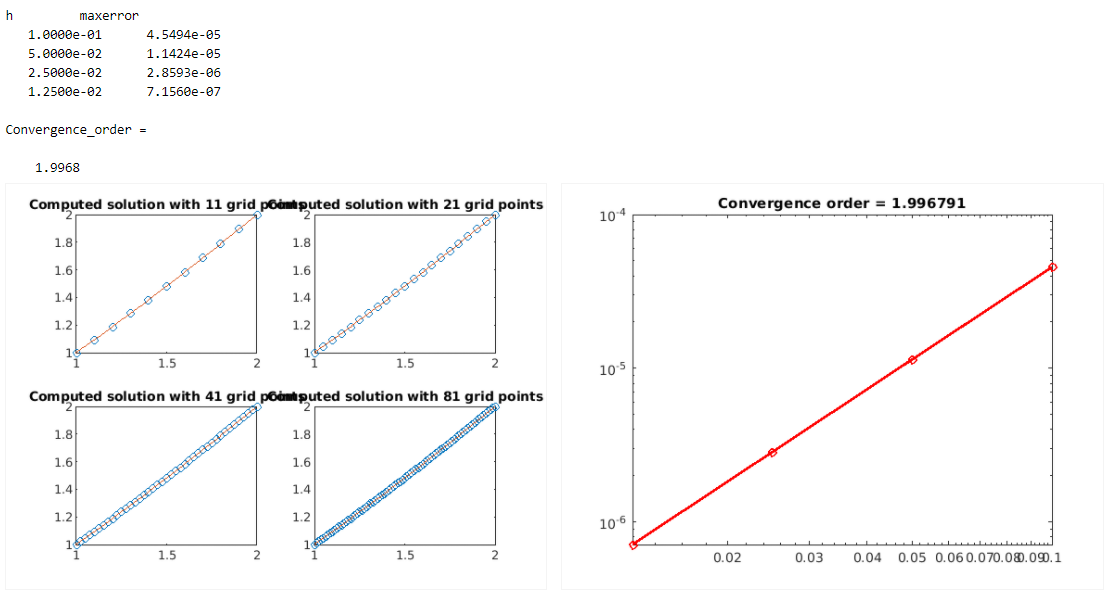
\includegraphics[scale=.5]{1c.PNG}
	\end{figure}
	\end{enumerate}


\end{enumerate}



\end{document}
